\documentclass[conference]{IEEEtran}

\IEEEoverridecommandlockouts
% The preceding line is only needed to identify funding in the first footnote. If that is unneeded, please comment it out.
%Template version as of 6/27/2024

\usepackage{cite}
\usepackage{amssymb,amsfonts}
\usepackage[fleqn]{amsmath}
\usepackage{algorithmic}
\usepackage{graphicx}
\usepackage{textcomp}
\usepackage{xcolor}
\usepackage{url}
\usepackage{here}
\usepackage[hang,small,bf]{caption}
\usepackage[subrefformat=parens]{subcaption}
\usepackage{stfloats} % プリアンブルに追加
\def\BibTeX{{\rm B\kern-.05em{\sc i\kern-.025em b}\kern-.08em
    T\kern-.1667em\lower.7ex\hbox{E}\kern-.125emX}}


\begin{document}

\title{Implementation of a VAE-Based Circuit for Image Compression and Anomaly Detection \\and Its Potential Use in Edge Computing\\
%{\footnotesize \textsuperscript{*}Note: Sub-titles are not captured for https://ieeexplore.ieee.org  and should not be used}
%\thanks{Identify applicable funding agency here. If none, delete this.}
}

\author{\IEEEauthorblockN{1\textsuperscript{st} Yuki Imamura}
\IEEEauthorblockA{\textit{Kyushu Institute of Technology} \\
\textit{School of Computer Science and Systems Engineering}\\
\textit{Department of Computer Science and Networks}\\
Fukuoka, Japan \\
imamura.yuuki475@mail.kyutech.jp}
\and
\IEEEauthorblockN{2\textsuperscript{nd} Taiga Kawasaki}
\IEEEauthorblockA{\textit{Kyushu Institute of Technology} \\
\textit{School of Computer Science and Systems Engineering}\\
\textit{Department of Computer Science and Networks}\\
Fukuoka, Japan \\
kawasaki.taiga711@mail.kyutech.jp}
}

\maketitle

\begin{abstract}
With the recent evolution of wireless communication technology and the spread of 5G, there is a need to create a new communication environment that takes advantage of the characteristics of low latency and multiple simultaneous connections.
On the other hand, there is a potential problem due to the increased burden of cloud processing.
Edge computing is attracting attention as a method to solve this problem.
In this study, we developed a system that compresses and analyzes acquired images by implementing VAE using FPGA to realize efficient data processing on an edge server.
As a result, the system was able to perform image compression and anomaly detection.
However, the system's performance is expected to be further improved by utilizing higher-accuracy FPGAs and by incorporating color image processing.
\end{abstract}

\begin{IEEEkeywords}
VAE, FPGA, Edge Computing, Image Compression, Anomaly Detection
\end{IEEEkeywords}

\section{Introduction}
In recent years, wireless communication technology has improved dramatically, and 5G communications are becoming increasingly popular.
Unlike conventional communication standards such as 4G, 5G has the three characteristics of “high speed and large capacity,” “low latency,” and “multiple simultaneous connections,” of which “low latency” and “multiple simultaneous connections” are important axes for building a new communication environment.
Conventional 4G communications have focused on smartphones and cell phones used by people.
However, 5G assumes that IoT devices such as vehicles, drones, and sensors will be connected to the network in large numbers.

In addition, cloud computing is the mainstream in the IT industry today\cite{jyotu-haku}.
As shown in the left side of Fig.\ref{fig:1-1}, the cloud performs the processing from the edge device and notifies the edge device of the result.
However, there is a limit to the amount of data acquired from many devices that can be processed only by the cloud, and the amount of traffic will increase, making it difficult to enjoy the benefits of 5G.

To solve these problems, edge computing has been gaining attention in recent years.
Edge computing is a technology that performs part of the processing that is conventionally performed in the cloud, such as data processing at a base station or server located near the user terminal (smartphone or IoT device)\cite{edge-com}\cite{nec-edge}.
Using this technique, it is possible to distribute the processing that is required in the cloud to edge computing, reduce the amount of communication traffic, and take advantage of the “low latency” that is one of the features of 5G.

\begin{figure}[tb]
    \begin{center}
        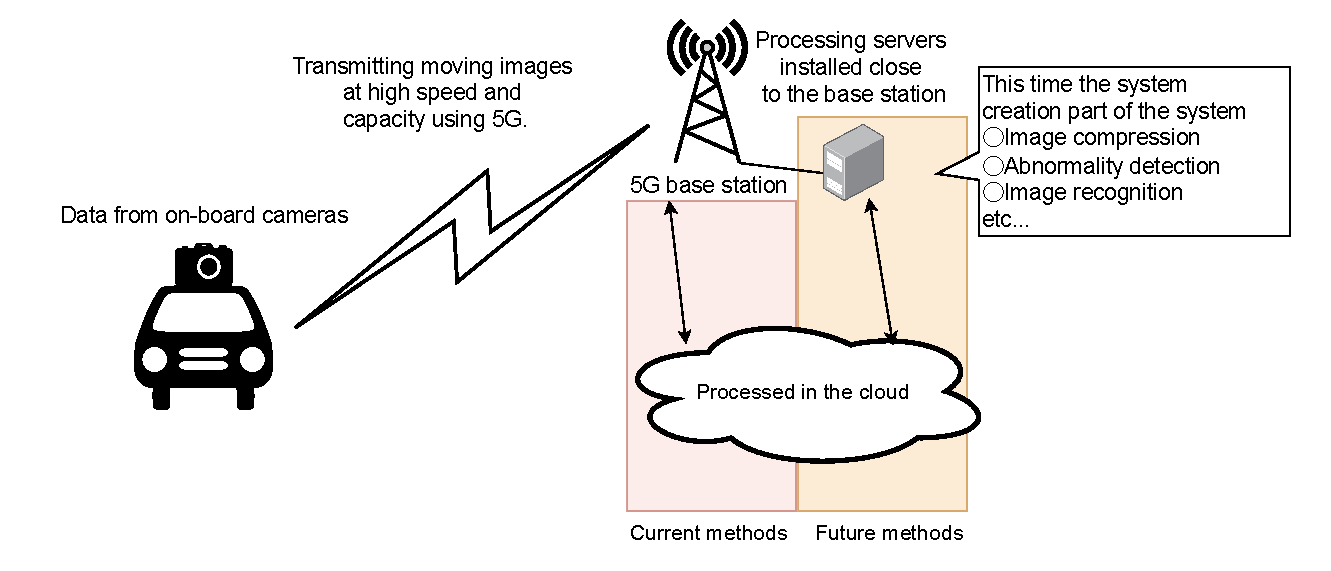
\includegraphics[width=0.98\columnwidth]{figures/Intr_1.pdf}
    \end{center}
    \caption{Image of edge computing and the part of the system created this time}
    \label{fig:1-1}
\end{figure}

Therefore, we considered the use of VAE and FPGAs to realize edge computing.
A system for detecting foreign objects on the road has already been created using VAE, and certain results have been obtained\cite{vae-road}. %References
Therefore, in this project, we aimed to create a part of the process on the right side of Fig.\ref{fig:1-1} by processing images acquired from an onboard camera using an FPGA equipped with a VAE.

\section{Method}
% 今回使用した環境を記載
The tools and their versions used in the creation of this system are shown in Table \ref{tb:1}.
ZYNQ-7010 with DIGILENT SoC is used as the FPGA evaluation board.
\begin{table}[tb]
    \centering
    \caption{Tools used in this development}
    \small
    \begin{tabular}{|c|c|} \hline
      Usage & tools used \\ \hline \hline
      For VAE simulation & MATLAB 2024b \\ \hline
      Hardware simulation & MATLAB/Simulink 2022a \\\hline
      HDL Code Generation & HDL Coder \\\hline
      FPGA Design Software & Vivado 2022.1 \\ \hline
      Hardware acceleration & Vitis 2022.1 \\\hline
      Evaluation Board & DIGILENT ZYNQ-7010 \\\hline
    \end{tabular}
    \label{tb:1}
\end{table}

\subsection{System Structure}
This VAE-equipped system has the following two functions.
\begin{itemize}
  \item[1] image compression\\
  The dimensional compression capability, one of the features of VAE, is applied to images.
  \item[2] Anomaly detection\\
  Another feature of VAE, anomaly detection is performed by comparing the original image and the generated image.  
\end{itemize}

This section describes the overall concept.
The images used in this project are grayscaled for simplicity.
The image is divided into blocks like a JPEG, and VAE is used for each block.
The block size is set to $16\times16$.
PSNR is used to compare the original image with the compressed image for each block.
Image compression and anomaly detection are processed using PSNR.
For image compression, if the PSNR is above a set threshold, the compressed latent space is used as the compressed data, since there is no problem in using the compressed latent space.
For anomaly detection, if the PSNR value is less than the threshold value, the system is set to judge the image as an anomaly because there is a high possibility that it is not a road.

In order to realize the above functions, the structure of VAE is described in\ref{2.2.3}.
The details of the FPGA structure are explained in \ref{2.2.4}, and finally the SoC FPGA structure is explained in \ref{2.2.5}.

\subsubsection{VAE Structure}\label{2.2.3}
A schematic of the VAE structure is shown in Fig.\ref{fig:2-2-2-1}.
Since $16 \times 16$ images are used, 256 input dimensions and 256 output dimensions were used in the design.
The latent space was designed to have 16 dimensions to allow for a certain degree of discrimination even after compression.
The encoder part uses a ReLU function for the mean and a soft plus function for the variance.
The decoder part uses a sigmoid function.
\begin{align}
  f(x) &= x &: ReLU function \label{sq:1} \\
  f(x) &= \log(1+e^x) &: Softplus function \label{sq:2}\\
  f(x) &= \dfrac{1}{1+e^{-x}} &: Sigmoid function \label{sq:3}
\end{align}

The VAE learning method is shown in Fig.\ref{fig:2-2-2-2}.
First, a large number of road-only blocks are prepared.
The blocks are used as teacher data to train VAE.
The learning conditions are summarized in table \ref{tb:2}.
In this case, we prepared a photo showing a road (the upper left image in Fig.\ref{fig:2-2-2-2}) and prepared the teacher data by converting the part showing only the road (the upper right image in Fig.\ref{fig:2-2-2-2}) into a block.
The VAE was trained in MATLAB, and the weights and parameters output from the training were used to control the VAE mounted on FPGA.

\begin{table}[b]
    \centering
    \caption{VAE learning conditions}
    \small
    \begin{tabular}{|c|c|} \hline
      epoch & 10000 \\ \hline
      eta & 0.0005 \\ \hline
      Layer2(number of latent spaces) & 16 \\ \hline
    \end{tabular}
    \label{tb:2}
  \end{table}

% VAEの構造図
\begin{figure}[tb]
    \begin{center}
      %Created by Kawasaki, Edited by Imamura
      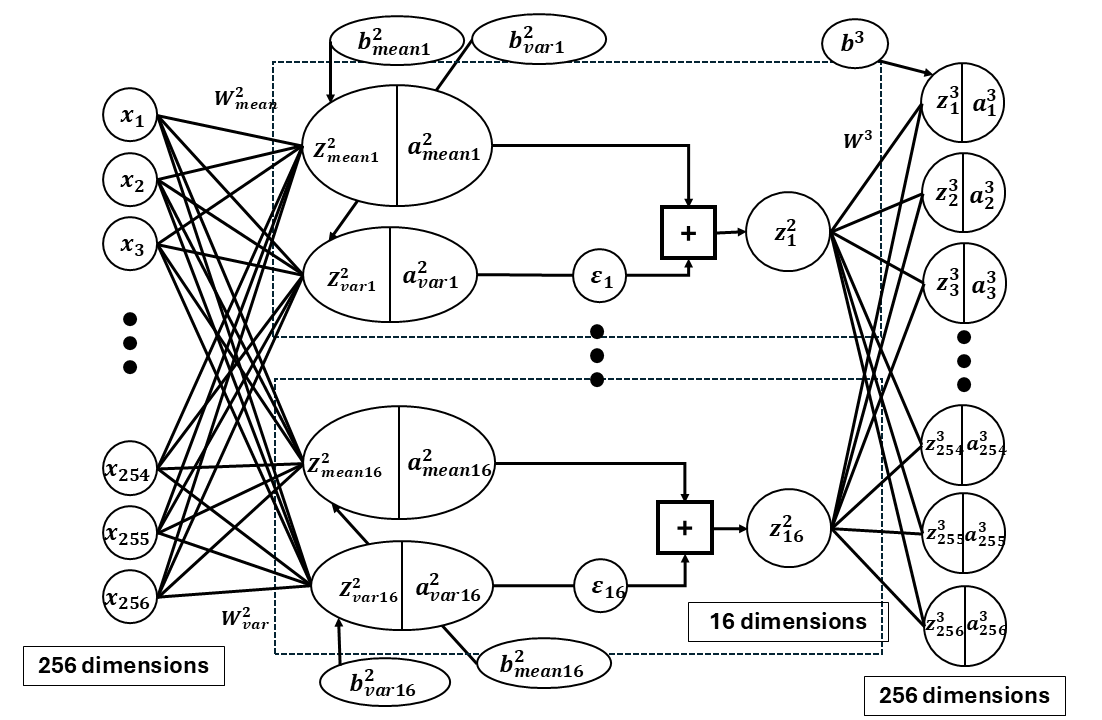
\includegraphics[width=0.98\columnwidth]{figures/VAE_1.png}
    \end{center}
    \caption{Structure of $256\times16\times256$VAE}
    \label{fig:2-2-2-1}
  \end{figure}
  
  \begin{figure}[tb]
    \begin{center}
      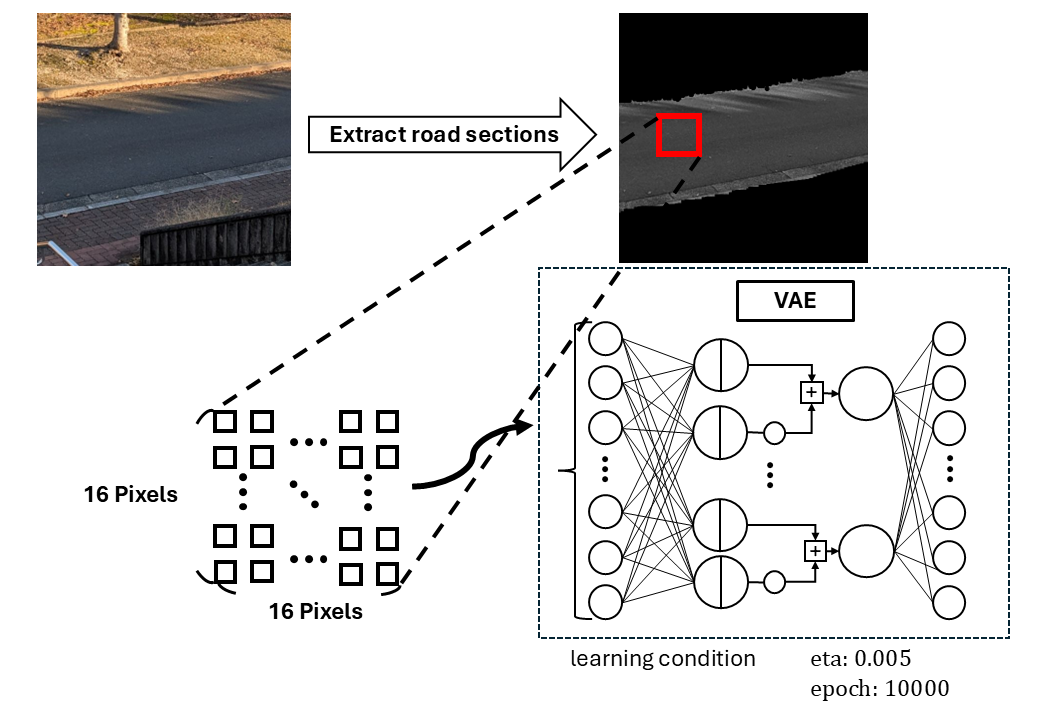
\includegraphics[width=0.98\columnwidth]{figures/VAE_2.png}
    \end{center}
    \caption{How to study VAE}
    \label{fig:2-2-2-2}
  \end{figure}

\subsubsection{FPGA Structure}\label{2.2.4}
The board used was ZYNQ-7010 manufactured by DIGILENT.
In this design, $X(16)$, $W(16\times2)$, and $b(16)$ were prepared as input data and $Z(16)$ as output as shown in Fig.\ref{fig:2-2-3-1} (the number of dimensions in parentheses).
The unit enclosed in the red box, where $Output_1$ is the output, performs the operation of multiplying the input and weight parameters, as shown in Equation \ref{sq:4}.
\begin{align}
  Output_1 = X_1 \times W1_1 \label{sq:4}
\end{align}
Sixteen such units are shown in the blue box.
The final $Z$ output is the computation of Equation \ref{sq:5}.
\begin{align}
  Z_1 = \sum_{i = 0}^{16} X_i \times W1_i + b1 \label{sq:5}
\end{align}

Initially, we wanted to put 256 input and 256 output operations on the FPGA, but there was a capacity limitation.
Therefore, we designed the VAE of $256\times16\times256$ to have 16 inputs for $X$ to make it easier to realize the VAE of $256\times16\times256$ that we designed this time.

% FPGA内の構造図
% エンコーダの中身
\begin{figure}[tb]
  \begin{center}
    %入力画像はPNG
    %created by Imamura
    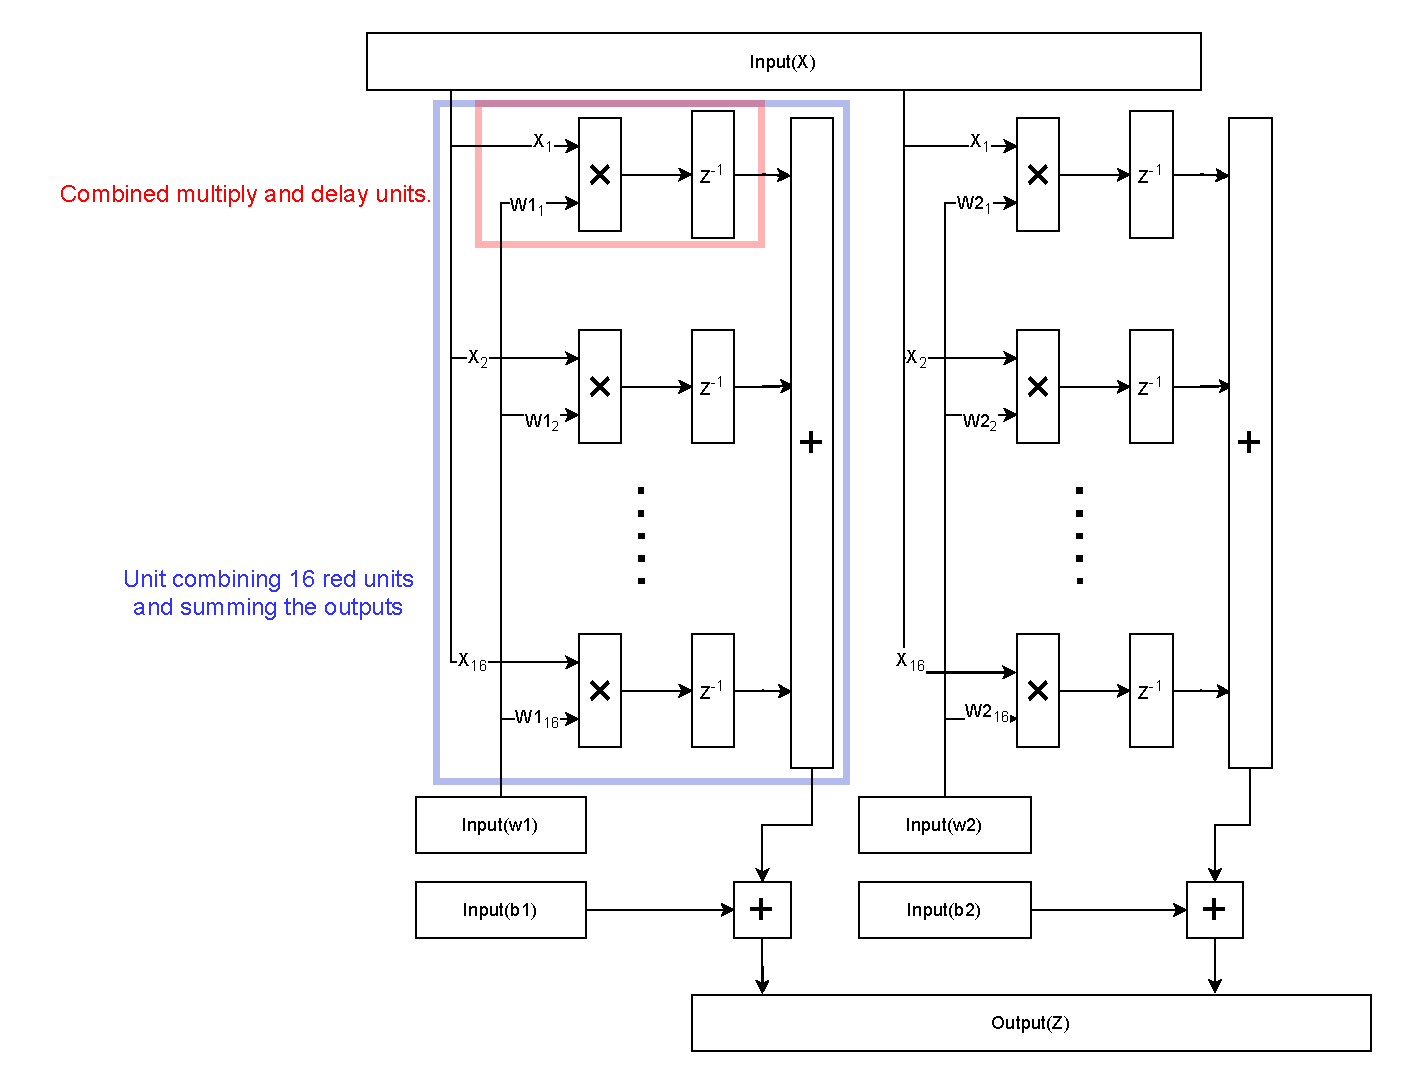
\includegraphics[width=0.98\columnwidth]{figures/FPGA_1.pdf}
  \end{center}
  \caption{FPGA structure}
  \label{fig:2-2-3-1}
\end{figure}

\subsubsection{SoC FPGA Structure}\label{2.2.5}
Fig.\ref{fig:2-2-4-1} shows an overview of the SoC FPGA system structure.
The processing \textbf{processing\_system7\_0} performs various processes through the bus, and plays the role of CPU.
The \textbf{dut\_forwa\_ip\_0} part is the part of the FPGA created this time.
The resource utilization evaluation after implementation is shown in Table \ref{tb:3}.

Next, an overview of the SoC FPGA processing is shown in Fig.\ref{fig:2-2-4-2}.
The SD card contains weights and parameters stored in CSV files and image data in RAW format.
The CPU reads these data.
The CPU then processes the input data according to the created FPGA and sends the data to the FPGA.
The FPGA executes the data as soon as it is stored and stores the output results.
The CPU reads the output result and processes the output data.
These processes are repeated.

This VAE is $256\times16\times256$, and the FPGA structure created in \ref{2.2.4} is $16\times2$.
The part of the FPGA that can be processed by running the designed FPGA once is shown in Fig.\ref{fig:2-2-4-3}.
The encoder assigns the computation of the two outputs to $z^2_{mean}$ and $z^2_{var}$.
Since the FPGA can process 16 out of 256 input dimensions in a single use, it is necessary to use the FPGA 16 times to compute a single latent space.
The output $z^2_{mean}$ and $z^2_{var}$ are designed to be stored in $b$.
Since there are 16 latent spaces, the encoder calculation runs a total of $16\times16=256$ times.
When computing the decoder part, only one FPGA run is needed to obtain 2 out of 256 dimensions of the output of the third layer $Z^3_i$.
Therefore, the FPGA is run 128 times in the decoder.
This kind of control was created using a CPU.

The $z^2_{mean}$, $z^2_{var}$, and $z^3$ obtained from the output are used to calculate $a^2_{mean}$, $a^2_{var}$, and $a^3$ using the active functions in the software.
Furthermore, $z^2$ is also calculated on the software using $a^2_{mean}$ and $a^2_{var}$.
Finally, PSNR is measured by comparing the input and output $a^3$ values.
\begin{table}[tb]
  \centering
  \caption{FPGA Resource Utilization}
  \small
  \begin{tabular}{|c|c|c|c|} \hline
    Resorce & Utilization & Available & Utilization[\%]\\ \hline
    LUT & 3301 & 17600 & 18.76 \\ \hline
    LUTRAM & 62 & 6000 & 1.03 \\ \hline
    FF & 3297 & 35200 & 9.37 \\ \hline
    DSP & 64 & 80 & 80.0 \\ \hline
    IO & 12 & 100 & 12.0 \\ \hline
    BUFG & 1 & 32 & 3.13 \\ \hline
  \end{tabular}
  \label{tb:3}
\end{table}

% SoC構造図
\begin{figure}[tb]
  \begin{center}
    %created by screenshot
    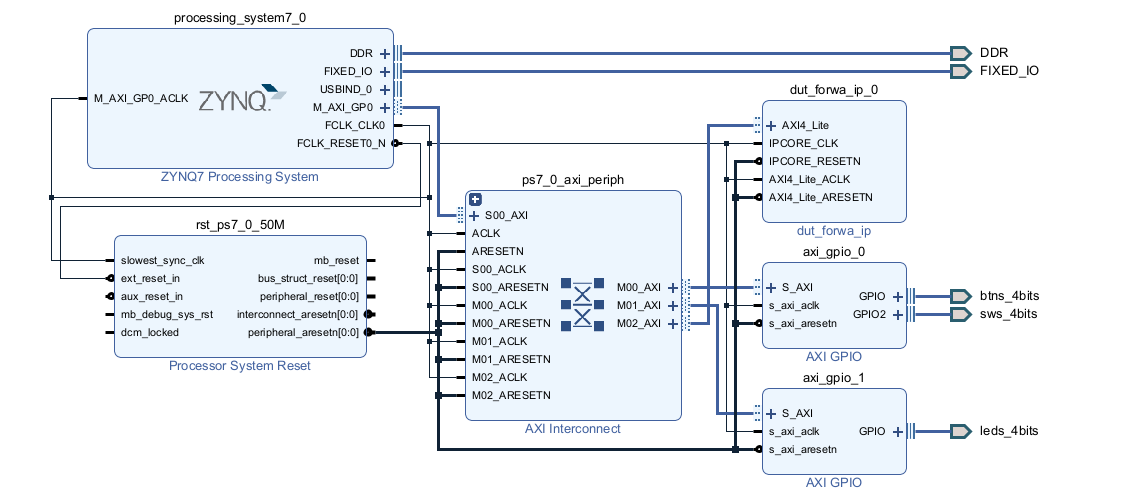
\includegraphics[width=0.98\columnwidth]{figures/SoC_1.png}
  \end{center}
  \caption{SoC FPGA Configuration Diagram}
  \label{fig:2-2-4-1}
\end{figure}

\begin{figure}[tb]
  \begin{center}
    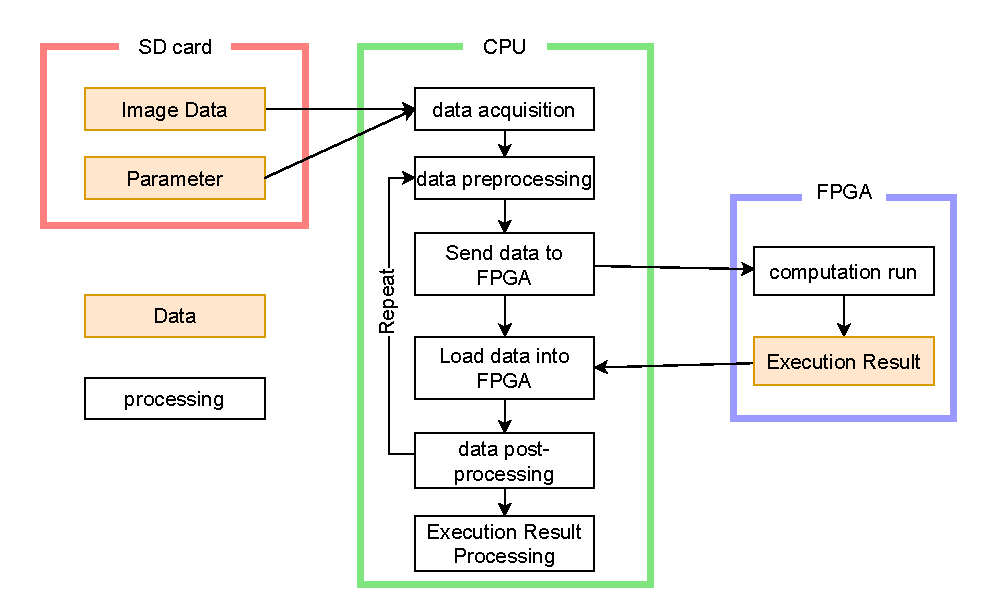
\includegraphics[width=0.98\columnwidth]{figures/SoC_2.pdf}
  \end{center}
  \caption{SoC FPGA Processing Overview}
  \label{fig:2-2-4-2}
\end{figure}

\begin{figure}[tb]
  \begin{center}
    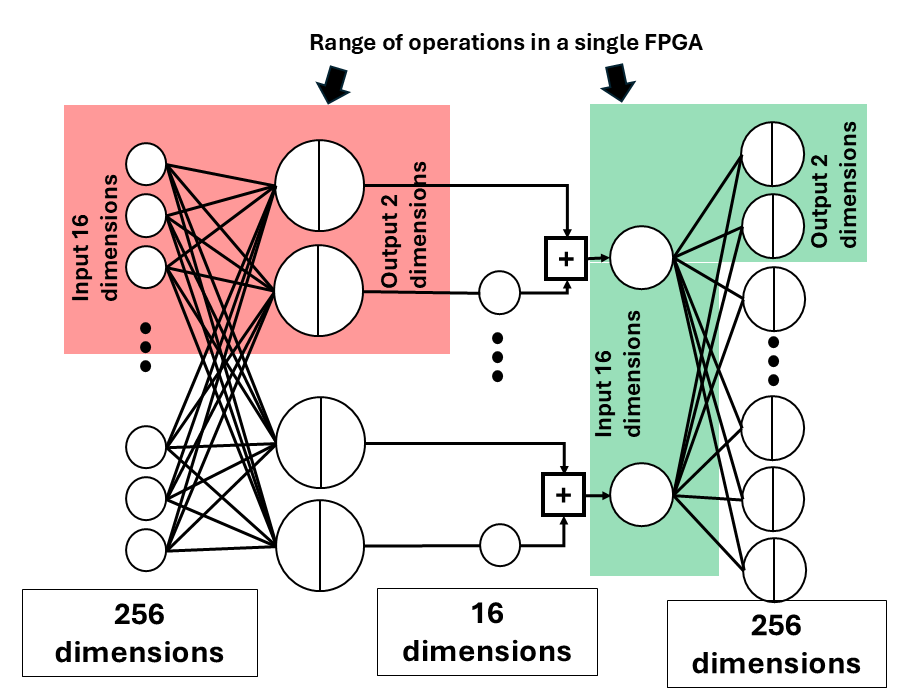
\includegraphics[width=0.98\columnwidth]{figures/SoC_3.png}
  \end{center}
  \caption{Image of FPGA use}
  \label{fig:2-2-4-3}
\end{figure}

\subsection{Experimental Procedure}
In this case, we prepared three types of images shown in Fig.\ref{fig:2-3-1}.
Fig.\ref{fig:2-3-2} is an image without any falling objects.
Fig.\ref{fig:2-3-3} and Fig.\ref{fig:2-3-4} are images with falling objects, and were prepared for comparison of anomaly detection.
The size of the image is $512\times512$, and the image is grayed out when passed through VAE.
The image is processed by dividing it into $16^times16$ blocks, and the PSNR is measured.
The PSNR is compared between the MATLAB output and the FPGA output.
The PSNR output from the FPGA is written to a CSV file, and the data is presented in MATLAB.

\begin{figure}[tb]
  \begin{minipage}[]{0.32\columnwidth}
    \centering
    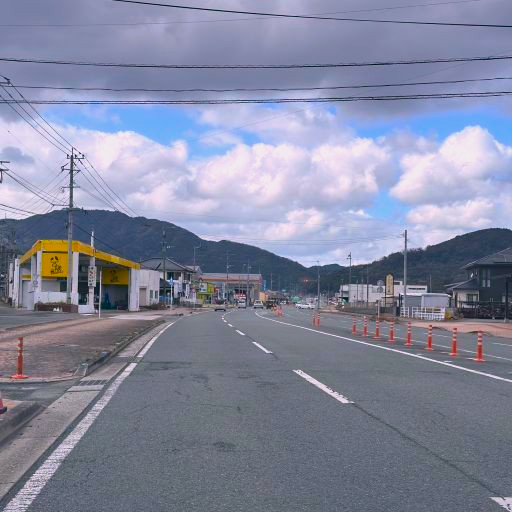
\includegraphics[width=0.9\columnwidth]{figures/Ex_pr1.png}
    \subcaption{Image 1\\Original image}
    \label{fig:2-3-2}
  \end{minipage}
  \begin{minipage}[]{0.32\linewidth}
    \centering
    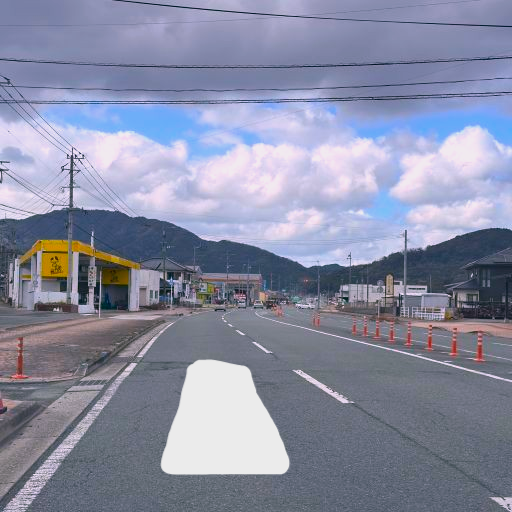
\includegraphics[width=0.9\columnwidth]{figures/Ex_pr2.png}
    \subcaption{Image 2\\With falling objects}
    \label{fig:2-3-3}
  \end{minipage}
  \begin{minipage}[]{0.32\linewidth}
    \centering
    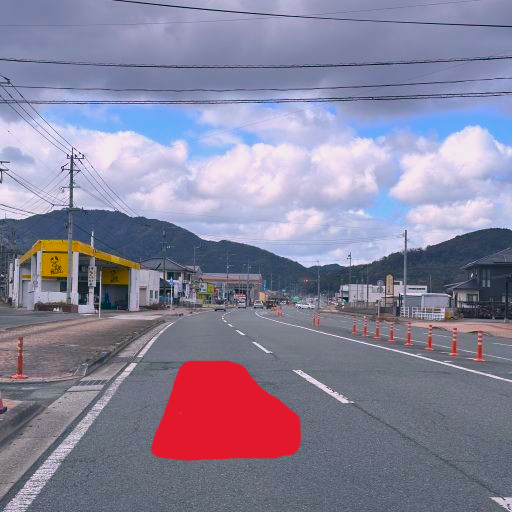
\includegraphics[width=0.9\columnwidth]{figures/Ex_pr3.png}
    \subcaption{Image 3\\With falling objects}
    \label{fig:2-3-4}
  \end{minipage}
  \caption{Evaluation image to be tested this time}
  \label{fig:2-3-1}
\end{figure}

\section{Experiments and Discussions}
\subsection{Experimental Results}
First, the SoC FPGA execution screen is shown in Fig.\ref{fig:3-1}.
The CSV file stored in the SD card is read by pressing button 0.
The image is passed through the VAE by pressing buttons 1 to 3.
Fig.\ref{fig:3-1} shows the state after button 0 is pressed and the parameters are acquired.

\begin{figure}
  \begin{center}
    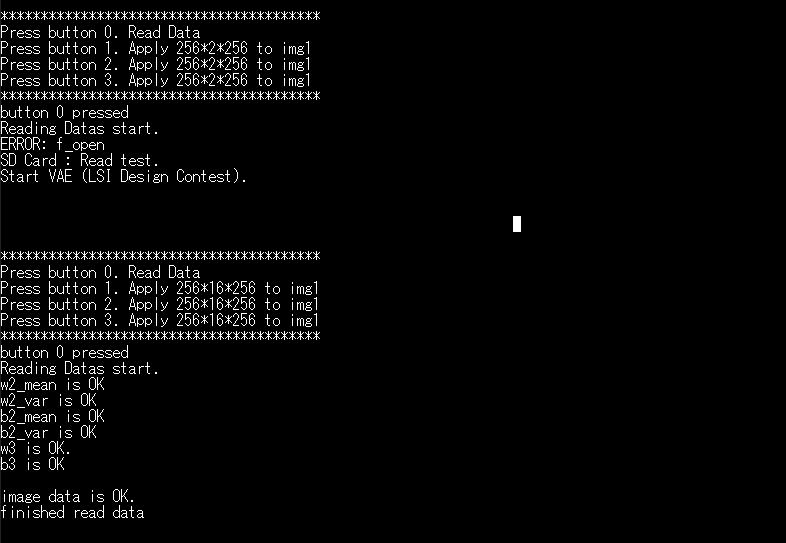
\includegraphics[width=0.98\columnwidth]{figures/Ex_re7.png}
  \end{center}
  \caption{SoC FPGA execution screen}
  \label{fig:3-1}
\end{figure}

\subsubsection{Comparison of output of image 1 }%Fig1
Fig.\ref{fig:3-1-3} shows the output in MATLAB and Fig.\ref{fig:3-1-4} shows the output in FPGA.
In MATLAB, the PSNR around the road area shows a value of 25 or higher.
In addition, parts of the sky and mountains also have a high PSNR.
The FPGA output shows a lower overall PSNR compared to MATLAB.
However, the PSNR of the road section is around 25, which is not a bad result.
\begin{figure}[tb]
  \begin{minipage}[t]{0.32\columnwidth}
    \centering
    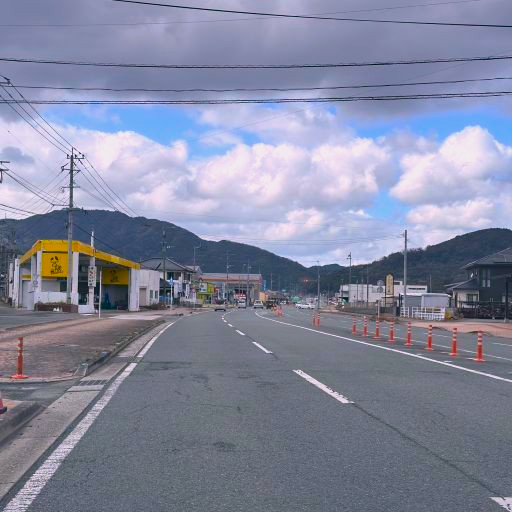
\includegraphics[width=0.9\columnwidth]{figures/Ex_pr1.png}
    \subcaption{Image 1 to be tested}
    \label{fig:3-1-2}
  \end{minipage}
  \begin{minipage}[t]{0.32\linewidth}
    \centering
    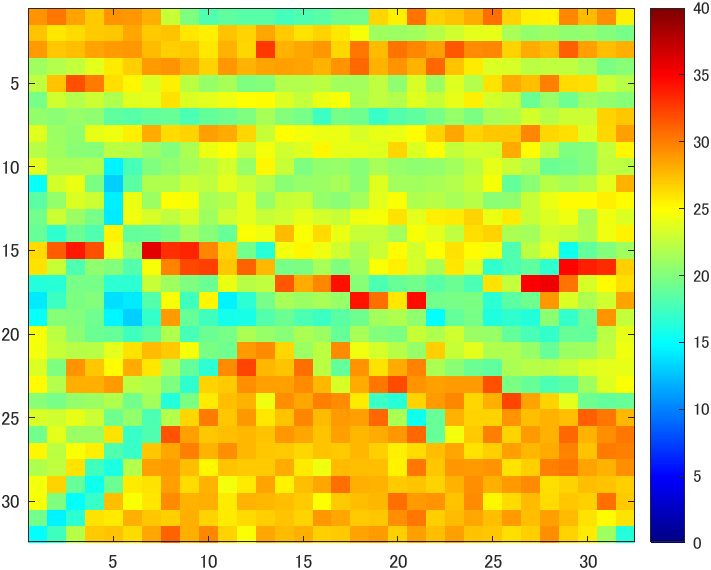
\includegraphics[width=0.9\columnwidth]{figures/Ex_re1.png}
    \subcaption{PSNR output block \\by block in MAT-\\LAB}
    \label{fig:3-1-3}
  \end{minipage}
  \begin{minipage}[t]{0.32\linewidth}
    \centering
    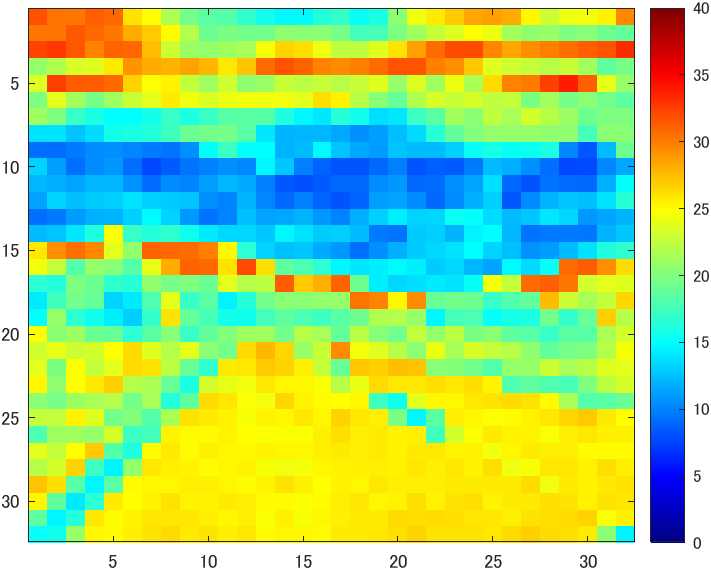
\includegraphics[width=0.9\columnwidth]{figures/Ex_re2.png}
    \subcaption{PSNR output block \\by block in FPGA}
    \label{fig:3-1-4}
  \end{minipage}
  \caption{Processing results for image 1}
  \label{fig:3-1-1}
\end{figure}

\subsubsection{Comparison of output of image 2 }%Fig2
Fig.\ref{fig:3-2-3} shows the output from MATLAB and Fig.\ref{fig:3-2-4} shows the output from FPGA.
Both MATLAB and FPGA outputs show a worse PSNR in the area of the falling objects.
\begin{figure}[tb]
  \begin{minipage}[t]{0.32\columnwidth}
    \centering
    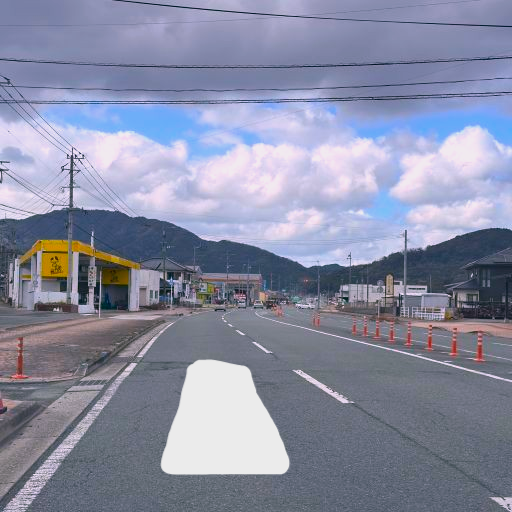
\includegraphics[width=0.9\columnwidth]{figures/Ex_pr2.png}
    \subcaption{Image 2 to be tested}
    \label{fig:3-2-2}
  \end{minipage}
  \begin{minipage}[t]{0.32\linewidth}
    \centering
    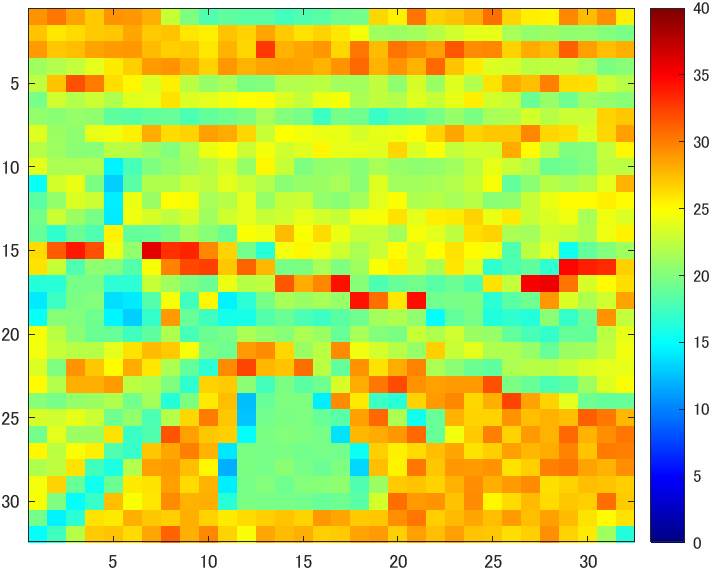
\includegraphics[width=0.9\columnwidth]{figures/Ex_re3.png}
    \subcaption{PSNR output block \\by block in MAT-\\LAB}
    \label{fig:3-2-3}
  \end{minipage}
  \begin{minipage}[t]{0.32\linewidth}
    \centering
    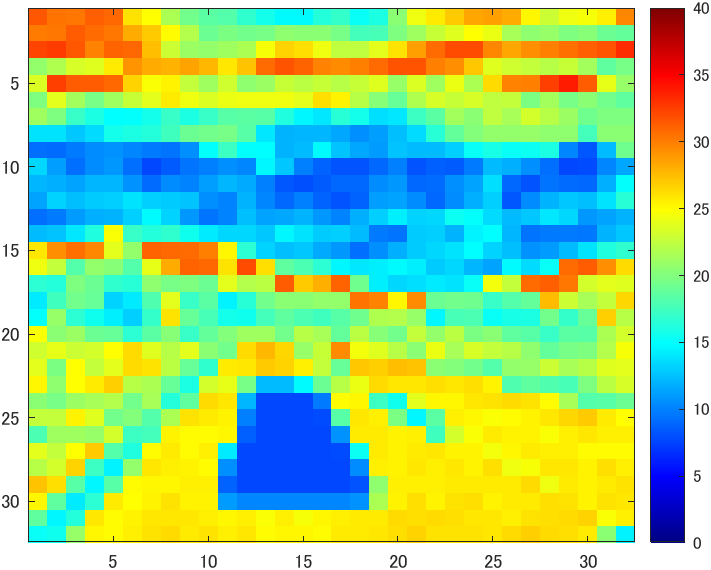
\includegraphics[width=0.9\columnwidth]{figures/Ex_re4.png}
    \subcaption{PSNR output block \\by block in FPGA}
    \label{fig:3-2-4}
  \end{minipage}
  \caption{Processing results for image 2}
  \label{fig:3-2-1}
\end{figure}

\subsubsection{Comparison of output of image 3 }%Fig3
Fig.\ref{fig:3-3-3} shows the output in MATLAB and Fig.\ref{fig:3-3-4} shows the output in FPGA.
Unlike the output in image 2, the PSNR in the area where the falling object is located is conversely improved.
\begin{figure}[tb]
  \begin{minipage}[t]{0.32\columnwidth}
    \centering
    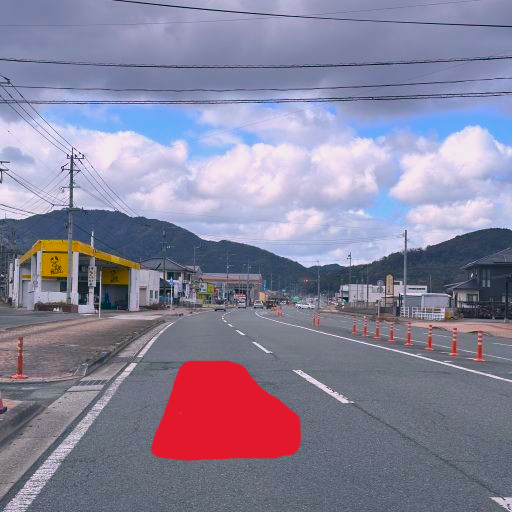
\includegraphics[width=0.9\columnwidth]{figures/Ex_pr3.png}
    \subcaption{Image 3 to be tested}
    \label{fig:3-3-2}
  \end{minipage}
  \begin{minipage}[t]{0.32\linewidth}
    \centering
    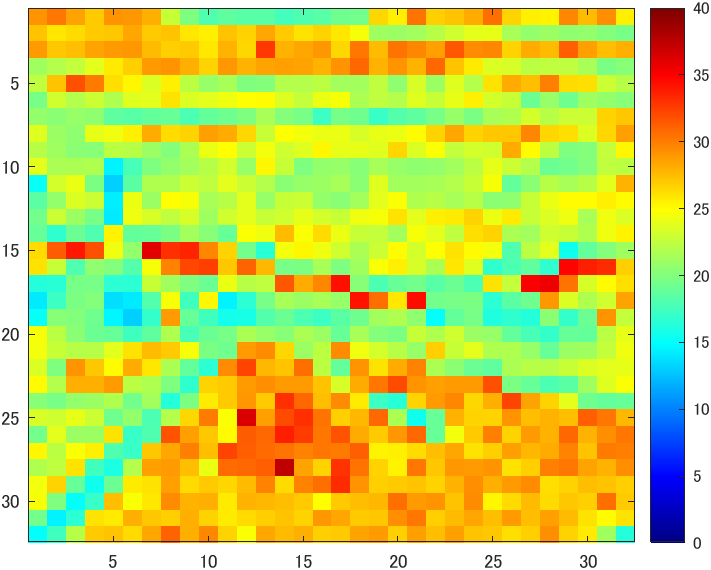
\includegraphics[width=0.9\columnwidth]{figures/Ex_re5.png}
    \subcaption{PSNR output block \\by block in MAT-\\LAB}
    \label{fig:3-3-3}
  \end{minipage}
  \begin{minipage}[t]{0.32\linewidth}
    \centering
    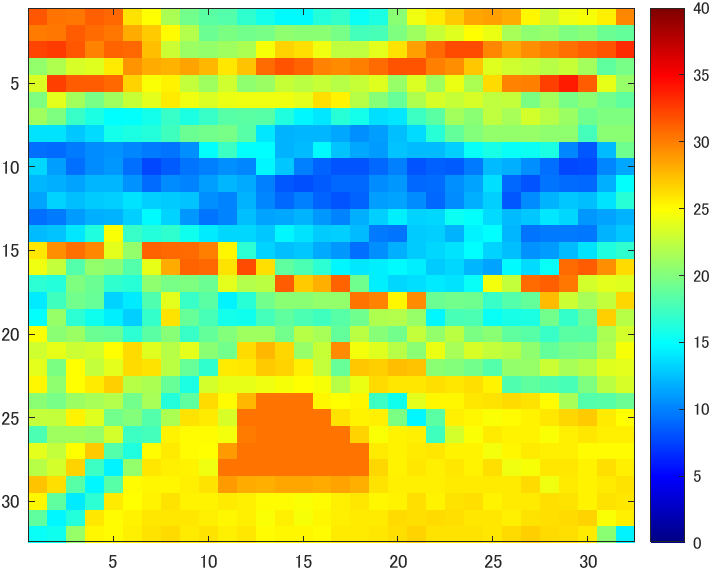
\includegraphics[width=0.9\columnwidth]{figures/Ex_re6.png}
    \subcaption{PSNR output block \\by block in FPGA}
    \label{fig:3-3-4}
  \end{minipage}
  \caption{Processing results for image 3}
  \label{fig:3-3-1}
\end{figure}

\subsubsection{Summary of results}
Comparing the output images, there were differences between the MATLAB and FPGA output results.
However, since the PSNR was higher for the road section in FPGA than for other sections, we do not think that there was a failure.

In addition, it was found that the anomaly detection was affected by the color of the falling object.
The PSNR worsened when the object was white, while the PSNR improved when the object was red.

\subsection{Consideration}
From the results obtained, the following three points are discussed.
\begin{enumerate}
  \item The point that PSNR is high except for roads \label{3-1-0}
  \item MATLAB and FPGA outputs are different \label{3-1-1}
  \item PSNR is improved even for red objects \label{3-1-2}
\end{enumerate}

(\ref{3-1-0}) can be considered from two points of view: the effect of grayscaling and the effect of VAE characteristics.
In particular, when the sky portion is grayscaled, it has fewer features than the road portion.
Therefore, the VAE created in this study can represent them, and it is thought that the image restoration capability of the VAE can be demonstrated.

(\ref{3-1-1}) is considered to be caused by the variables used and the fixed-point error.
However, since the detailed output has not been confirmed, we will conduct further verification to determine the cause.

(\ref{3-1-2}) is thought to be caused by grayscaling.
When the red color was converted to grayscale, it was almost the same as the color of the road (Fig.\ref{fig:3-3-5}).
This suggests that the color scale should be used to correctly identify falling objects.

\begin{figure}
  \begin{center}
    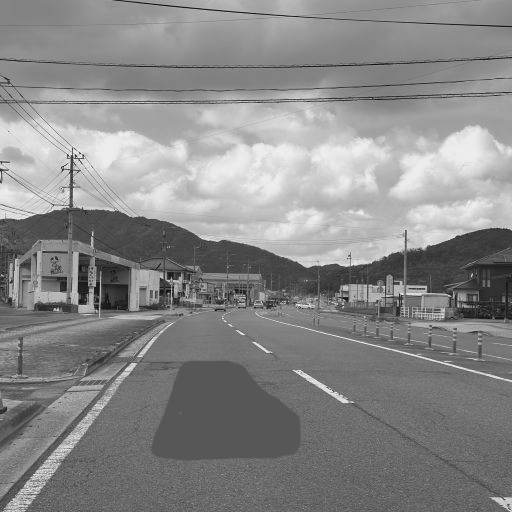
\includegraphics[width=0.45\columnwidth]{figures/De_re1.png}
  \end{center}
  \caption{Image 3 converted to grayscale}
  \label{fig:3-3-5}
\end{figure}

\subsubsection{Evaluating adoption in edge computing}
We will evaluate whether it can be adopted as edge computing.

First, we evaluate image compression.
This time, the PSNR threshold is set at 25, and judgments are made on the basis that images above the threshold are compressible and those below the threshold are uncompressible.
The number of blocks for which the threshold is 25 or higher, the capacity before compression, the capacity after compression, and the compression ratio are shown in Table \ref{tb:4}.
The size calculation is shown in the formula (\ref{sq:10}).
Since the original image takes values from 0 to 255, each pixel is 8 bits.
Since the latent space is compressed data, 8-bit fixed-point numbers are used.
The $B$ denotes the number of blocks above the threshold.
\begin{align}
  size = B \cdot 16 \cdot 8[bit] + (32\cdot32 - B) \cdot 16 \cdot 8[bit] \label{sq:10}
\end{align}
The compression ratio for all the images is close to 70\%.
By sending compressed images to the cloud for processing, it is possible to reduce the amount of traffic from the base station to the processing server and to improve the processing speed in the cloud.

Next, anomaly detection is evaluated.
As shown in the experimental results, whether an abnormality can be detected depends on the color of the falling object.
However, since abnormality detection is possible when the object is white, we believe that it is possible if the processed image is a color image.
If the recognition is performed on the area where the vehicle is going to run, it is possible to avoid accidents by immediately notifying the vehicle of the recognition results.

Finally, we evaluate real-time performance, which is important in edge computing.
The system took about 4 to 5 seconds to input an image and output the PSNR.
If the system were to continue at this rate, an accident could occur before an abnormality judgment could be made.
The reason for the long processing time is thought to be that data was written and read many times using a time-consuming bus.
In this case, the circuit that could be mounted on the FPGA is a part of VAE, and the FPGA is executed many times, and data is transferred using the bus each time.
In fact, to process a $512\times512$ image in VAE, the FPGA is run $393216$ times.
However, it is highly possible that this problem can be solved by using a higher-precision FPGA.

\begin{table}[t]
  \centering
  \caption{image compression effect}
  \small
  \begin{tabular}{|c|c|c|c|c|} \hline
    No. & Blocks & Before[bit] & After[bit] & Com.ratio[\%]\\ \hline
    1 & 346 & 2097152 & 1432832 & 68.32 \\ \hline
    2 & 305 & 2097152 & 1511552 & 72.08 \\ \hline
    3 & 349 & 2097152 & 1427072 & 68.05 \\ \hline
  \end{tabular}
  \label{tb:4}
\end{table}

\section{Conclusions and Future Prospects}
In this study, we implemented VAE on FPGA and constructed a system that compresses road images and detects anomalies.
The results show that image processing in edge computing using FPGAs is feasible.

Although the system has some problems, we believe that they can be solved with appropriate improvements.
Therefore, we believe that the system has potential for future industrial applications.

This contest allowed us to experience LSI development using FPGAs.
I felt the future potential of FPGAs and recognized that FPGAs are necessary devices for efficient computation in today's world where AI is used on a daily basis.
I would like to continue to develop FPGAs that can demonstrate their capabilities, and since technologies for developing FPGAs, such as high-level synthesis, are evolving day by day, I would like to challenge myself in various ways.

\section*{Acknowledgment}
Thank you to the LSI Design Contest Executive Committee for organizing this contest, and to the organizers, co-sponsors, sponsors, and supporters for their support.
I would also like to thank all the professors who provided various kinds of support even though they were not assigned to my laboratory.

\begin{thebibliography}{10}
\bibitem{5g} 
H. Morikawa, \textit{5G Jisedai Ido Tsushin Kikaku no Kanosei}, Iwanami Shoten, Tokyo, 2020.
\bibitem{edge-com} 
Y. Tanaka, N. Takahashi, and R. Kawamura, "IoT Jidai o Hiraku Edge Computing no Kenkyu Kaihatsu," \textit{NTT Giho Journal}, vol. 27, no. 8, pp. 59-63, 2015.
\bibitem{nec-edge}
H. Yokota, S. Oda, T. Kobayashi, D. Ishii, T. Ito, and A. Isozumi, "IoT no Missing Link o Tsunagu Edge Computing Gijutsu," \textit{NEC Giho}, vol. 70, no. 1, 2017.
\bibitem{jyotu-haku}
Ministry of Internal Affairs and Communications, "Reiwa 6-nenban Joho Tsushin Hakusho," 2024.
\bibitem{vae-road}
T. Yamamoto, A. Hashimoto, and H. Okamoto, "Heikin Gazou ni Taisuru VAE Ijou Kenshi no Tekiyo ni Yoru Doro Rakka-mono Kenshutsu," in \textit{Proc. Annu. Conf. Jpn. Soc. Artif. Intell.}, vol. 35, 2021.
\bibitem{LSI}
"LSI Design Contest," Available: \url{http://www.lsi-contest.com/}. Accessed: 2025-01-31.
\end{thebibliography}
\vspace{12pt}
%\color{red}
%IEEE conference templates contain guidance text for composing and formatting conference papers. Please ensure that all template text is removed from your conference paper prior to submission to the conference. Failure to remove the template text from your paper may result in your paper not being published.

\end{document}
